% Created 2018-12-09 Sun 11:03
% Intended LaTeX compiler: pdflatex
\documentclass[11pt]{article}
\usepackage[utf8]{inputenc}
\usepackage[T1]{fontenc}
\usepackage{graphicx}
\usepackage{grffile}
\usepackage{longtable}
\usepackage{wrapfig}
\usepackage{rotating}
\usepackage[normalem]{ulem}
\usepackage{amsmath}
\usepackage{textcomp}
\usepackage{amssymb}
\usepackage{capt-of}
\usepackage{hyperref}
\date{Sat Dec  8 11:19:50 +0545 2018}
\title{Computer Security lab 2018 ( Bufferoverflow lab)}
\hypersetup{
 pdfauthor={},
 pdftitle={Computer Security lab 2018 ( Bufferoverflow lab)},
 pdfkeywords={},
 pdfsubject={},
 pdfcreator={Emacs 26.1 (Org mode 9.1.9)}, 
 pdflang={English}}
\begin{document}

\maketitle
Buffer overflows exploits occur when a program s to write into a buffer beyond the buffers size and get arbitrary code to execute. This can lead to bypassing security protocols, executing parts of code that aren't meant to be executed (changing the flow of control), or gaining control of a machine.

\section*{Setup}
\label{sec:org015974e}
To disable address randomization in kernel, for ease of bufferoverflow test
\begin{verbatim}
# to rollback set value to 2
sudo sysctl -w kernel.randomize_va_space=0
\end{verbatim}
Also \textbf{gcc} compiler implements a security mechanism called \texttt{stack guard} to disable it you can use a flag \texttt{-fno-stack-protector} during compilation

\section*{Tools}
\label{sec:org25e1701}
\subsection*{objdump}
\label{sec:org3fc7df8}
This is a simple tool that will dump an object files information. This will parse the object file and give information on mapped memory for functions, symbols, header information, etc.

\section*{Tasks}
\label{sec:orgccbcd43}
\subsection*{2.1 man objdump}
\label{sec:org9840cf8}
\subsubsection*{Answers}
\label{sec:org8806435}
\begin{itemize}
\item \texttt{-x or -{}-all-headers} (Display all available header information, including the symbol table and relocation entries.  Using -x is equivalent to specifying all of -a -f -h -p -r -t.)
\item \texttt{-t or -{}-syms} (Print the symbol table entries of the file.)
\item \texttt{-M intel or -{}-disassembler-options=intel} ( where M is the flag and \texttt{intel} is argument )
\end{itemize}
\subsubsection*{Sample Example and answers}
\label{sec:org05e3846}
\uline{Sample C program}
\begin{verbatim}
int add_nums(int a, int b){
return a + b;
}

int main(void){
add_nums(17, 25);
}
\end{verbatim}
\begin{itemize}
\item Answers according to my machine
\label{sec:org29b98c5}
\begin{itemize}
\item bytecode for ret is \texttt{c3}
\item memory location of main function is \texttt{000000000000112d}
\item memory location of add\(_{\text{num}}\) func is \texttt{0000000000001119}
\item \texttt{push} and \texttt{mov} are the two assembly instruction
\end{itemize}
\end{itemize}

\subsection*{2.2 GDB}
\label{sec:orgcd5e49b}
GDB is a debugging tool that allows you to run the compiled file and step through the assembly. Before we look at the simple.c file with gdb, here is a table of common commands.
\subsubsection*{Answers}
\label{sec:org5cba0cb}
\begin{itemize}
\item \texttt{0x0000555555555140} memory address after the call to add\(_{\text{nums}}\)
\item 
\end{itemize}
\subsection*{3.1 Simple Buffer Overflow}
\label{sec:org221debd}
\subsubsection*{Answer}
\label{sec:org1315fe1}
\begin{itemize}
\item buffer\(_{\text{one}}\)=one, buffer\(_{\text{two}}\)=two, value=5 and after buffer\(_{\text{one}}\)=one, buffer\(_{\text{two}}\)=1234, value=5
\item I used "12345678910"
\item buffer\(_{\text{two}}\)=12345678910 value and buffer\(_{\text{one}}\)=910 (my \texttt{buffer\_two} and \texttt{buffer\_one} was 8 byte big)
\begin{center}
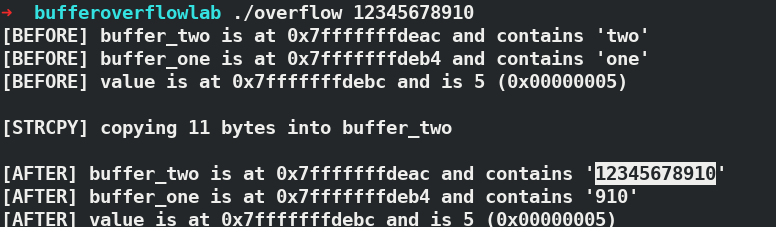
\includegraphics[width=.9\linewidth]{./bof_run.png}
\end{center}p
\item I got this error after I kept long value: \texttt{Program received signal SIGSEGV, Segmentation fault. 0x0000003432343332 in ?? ()}
\begin{center}
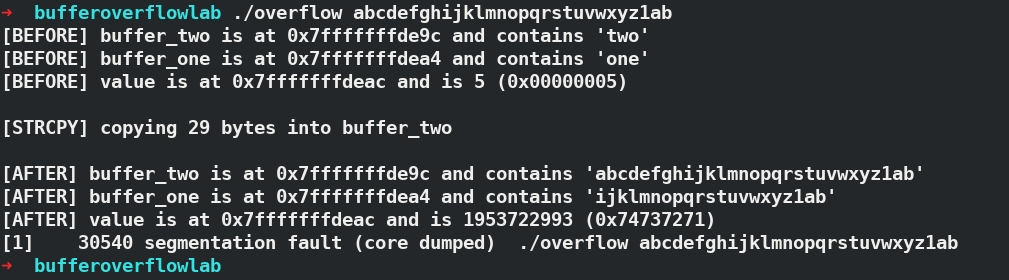
\includegraphics[width=.9\linewidth]{./bof_error.png}
\end{center}
\item previously buffer\(_{\text{one}}\)"one", buffer\(_{\text{two}}\)="two", value=5, after buffer\(_{\text{one}}\)="ijklmnop", buffer\(_{\text{two}}\)="abcdefghijklmnop", value=""(empty)
\end{itemize}
\begin{center}
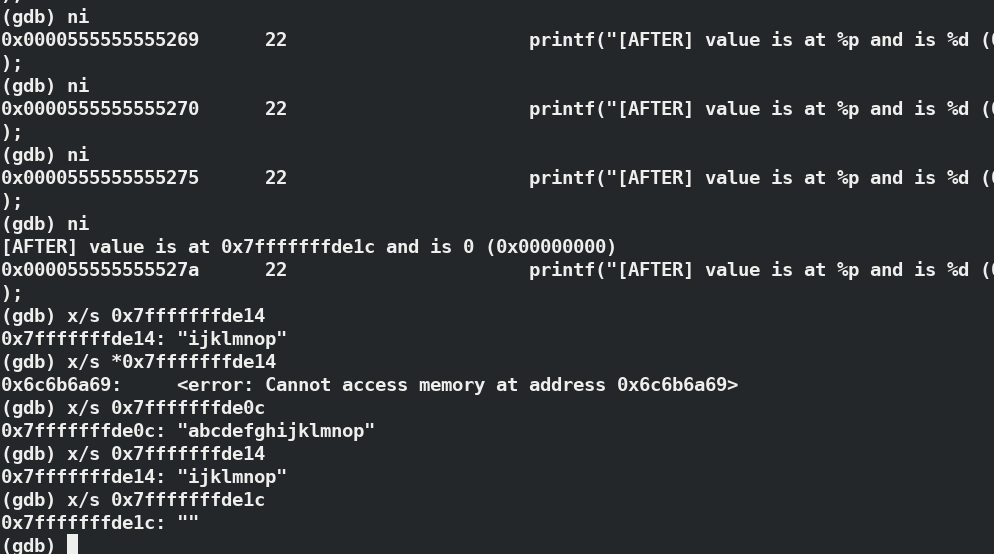
\includegraphics[width=.9\linewidth]{./bof_one_two.png}
\end{center}
\begin{itemize}
\item the following output was seen by running with fullalphabet \texttt{./overflow 'abcdefghijklmnopqrstuvwxyz'}
\begin{center}
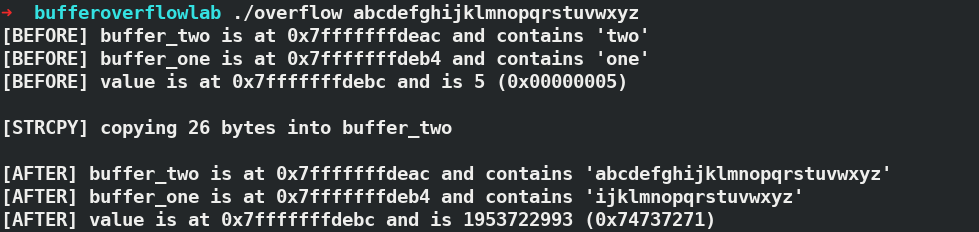
\includegraphics[width=.9\linewidth]{./bof_full_alpha.png}
\end{center}
\item Significance about above command is that, whenever the input is given more than 8 bytes it overflows towards next buffer regardless of any change in memory addresses.
\end{itemize}
\end{document}
